%!TEX root = ../Main.tex

\chapter{Genetic map of \textit{Yr15} with RNA-Seq}
\label{yr15}
%This section describes in detail than the paper of \citet{Ramirez-Gonzalez-2014}
 
%Breeding importance of \textit{Yr15} and original source (an introgression of \textit{T. diccocoides}). 
Wheat breeding programs aim to improve the wheat lines available for production. 
One of the traits desired in an elite line is the resistance to pathogens, such as \textit{Puccinia striiformis} f. sp.  \textit{tritici}, the fungi responsible of yellow rust.
A source of resistance genes is are introgressions from other species, suchas \textit{Triticum diccocides}. 
In the University of Sydney a collection of Near Isogenic Lines (NILs) with introgressions to several Yellow Rust resistance genes on a susceptible background were developed \citep{Wellings1998}. 
On this chapter the NIL for the \textit{Yr15} locus is used to produce a mapping population to improve diagnostic markers. 
The population was sequenced using RNA-Seq and a bioinformatic pipeline was developed to score Single Nucleotide Polymorphisms (SNPs) linked to the \textit{Yr15} locus.  
Finally, the best candidate SNPs where selected to produce a genetic map which lead to a triplet of markers diagnostic to the target locus. The results of this chapter are published in \citet{Ramirez-Gonzalez-2014}.

\section{Mapping population}
To   

\begin{wrapfigure}[15]{R!}{6cm}
    \centering
     \begin{subfigure}[b]{2.8cm}
        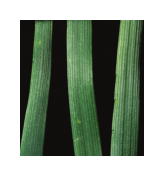
\includegraphics[width=1\textwidth]{Yr15/Figures/population/Yr15Photo.pdf}
        \caption{}
        \label{fig:yr15.yr15Photo}
    \end{subfigure}
    ~
    \begin{subfigure}[b]{2.8cm}
        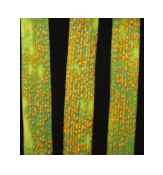
\includegraphics[width=1\textwidth]{Yr15/Figures/population/AVSPhoto.pdf}
        \caption{}
        \label{fig:yr15:avsPhoto}
    \end{subfigure}

    \begin{subfigure}[b]{6cm}
        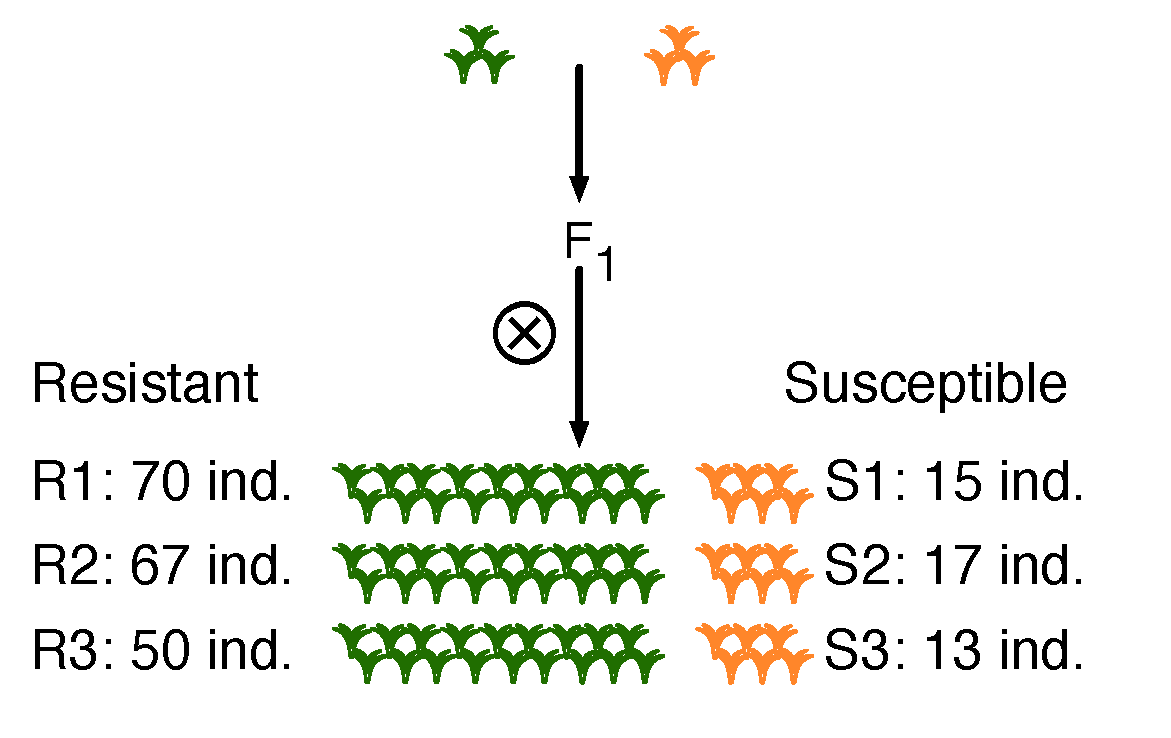
\includegraphics[width=1\textwidth]{Yr15/Figures/population/F2Population.pdf} 
        \caption{}
        \label{fig:yr15:F2Pop}
    \end{subfigure}
    \caption{ (\subref{fig:yr15.yr15Photo}) Avocet(Sydney) + \texttt{Yr15}. (\subref{fig:yr15:avsPhoto}) Avocet (JIC), succeptible to Yellow Rust.  (\subref{fig:yr15:F2Pop}) $F_{2}$ population}
\end{wrapfigure}

\section{Sequencing and mapping} 

RNA-Seq and the decision to call SNPs on gene models rather than the whole reference.  Details of the mapping against the Wheat UniGenes \cite{PontiusJUWagnerL2002} and the UCW. \cite{Krasileva2013} gene models.  

\section{SNP Calling}. 
\verb|Ruby| implementation of the methodology described by \citet{Trick2012}. 

\section{Bulk Frequency Ratios} 
Results of the simple SNP calls from the progenitors and how the score of the Bulk Frequency Ratios(BFR) improve the location of the SNPs. 

\section{\textit{In silico} mapping}
Mapping of the gene models to the IWGSC CSS \cite{Mayer2014} reference and the location of the SNPs using the genetic map from \citet{Wang2014}.

\section{Assay selection}. 
The selection criteria to decide which SNPs where selected to produce the genetic map: BFR$>$6, in the short arm of chromosome group 1 and from the \textit{Yr15} progenitor.

\section{Genetic map} 
\label{yr15:geneticMap}
The three versions of the genetic map: With a subset of the F\textsubscript{2} population

\section{Assembly of the transcriptome} 
A comparison between thef known unigenes and the transcript from the progenitors. Since \textit{Yr15} comes from an introgression with \textit{T. diccocoides}, some novel transcripts can be extracted. Analysis of the gels from Mitaly? 

\section{Conclusions} 
Remarks on how this techinque can be used to do fine-mapping and that if I were to start the project now I would  use exome capture or Ren-Seq. 